\documentclass[10pt,a4paper]{article}
\usepackage[latin1]{inputenc}
\usepackage{amsmath}
\usepackage{amsfonts}
\usepackage{amssymb}
\usepackage{graphicx}
\usepackage{float}
\usepackage{soul}
\usepackage{caption}
\usepackage{subcaption}
\usepackage[section]{placeins}
\usepackage[left=2cm,right=2cm,top=2cm,bottom=2cm]{geometry}
\author{Akshat Mahajan}
\title{Physics 180Q - Lab Report 4}
\begin{document}
\maketitle

\textsl{This lab was performed in conjunction with Hanwen Qin. The variable impedance terminator was set to 10 k$\Omega$ throughout, as analysis of the results from Week 1 had demonstrated that it gave the most accurate responses overall.}

\section*{Part 1: Coupling into a Single Mode Fiber}

In this section, we measured the beam profile, noted the optical characteristics of the collimator and optical single-mode fibre, and designed a two-lens telescope to minimise our beam waist to about the half the numerical mode aperture of the optical fibre.

\begin{itemize}
\item If you have not already measured the profile of the raw laser beam, do so now.

\textbf{Answer: } See the following figures. From Week 3, the beam waist was found to be about 0.2 mm along the $x$-axis and about 0.5 mm in the $y$-axis. In the interest of time, we assumed a similar behaviour would exist this time and chose to characterise the beam purely along the $x$-axis; since the beam waist after the collimator is inversely proportional to the beam waist before it, we reasoned that, if we could get the beam waist in the $x$-direction to be about as small as the desired beam waist, then the beam waist in the $y$-direction would also be small enough to fit into the optical fiber. 

The beam waist along the $x$-axis was found to be about 0.945 mm this time around. 

\begin{figure}[H]
\centering
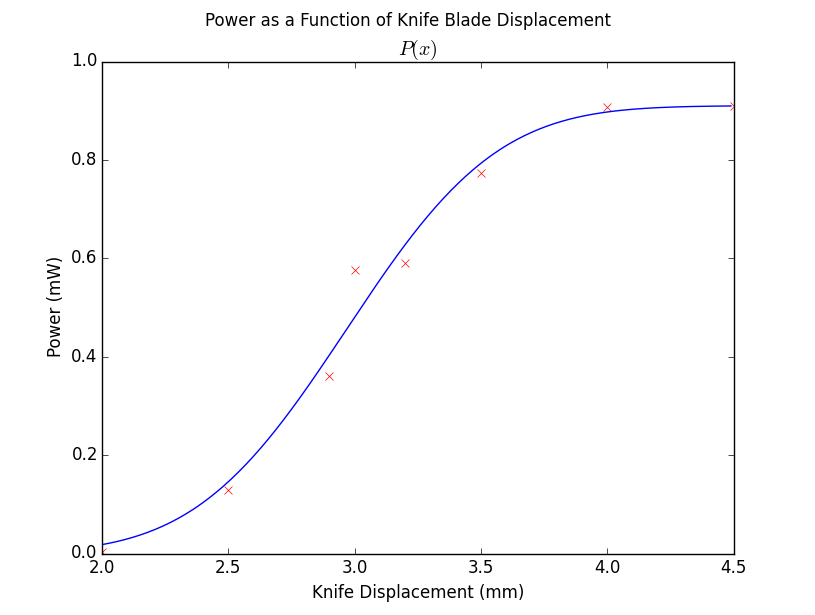
\includegraphics[scale = 0.5]{../Analysis/beam_profile_init.png}
\caption{Beam profile prior to telescope and collimator}
\end{figure}

\item Find the single mode fiber, and look up its specifications. The important parameters are Numerical Aperture and Mode Field Diameter (MFD).

\textbf{Answer: }The single mode fiber is a Thorlabs SM600. The Mode Field Diameter can vary anywhere between 3.6 - 5 $\mu$m at 633 nm (which we extrapolate to 670 nm), so our desired beam waist should be at the most 2.5 $\mu$m. The numerical aperture can also vary anywhere between 0.1 to 0.14. 

\item Using the focal lengths of fiber collimators available in the lab, use equation 7 from Week 3 to estimate the beam diameter needed to achieve the desired spot size on the fiber.

\textbf{Answer: }The focal length of our chosen single-mode fibre is 4.6 mm. Our desired waist is about 2.5 microns across. Our beam's wavelength is about 670 nm. Eq. 7 tells us that our waist just before the collimator should be about

$$w_{02} = \dfrac{\lambda f}{w_{01}n\pi} = \dfrac{670 \times 10^{-9} \times 4.6 \times 10^{-3}}{3.14 \times 2.5 \times 10^{-6}} = 0.392 \times 10^{-3} = 0.4 \,\mathrm{mm}$$

\item Design a 2 lens telescope that will get you close [to the desired beam length].

\textbf{Answer: }The desired magnification of our beam is about 0.9/0.4 = 2.25; the closest magnification we could achieve with existing focal lengths was about $ = \dfrac{f_{o}}{f_{e}} = $ 75mm /40 mm = 1.875. Hopefully, beam convergence thereafter would allow us to do the rest. \\

We set up two beam-steering mirrors and a two-lens telescope system of objective focal length 75 mm and eyepiece 40 mm. As we'll see in the next section, it worked remarkably well!
\end{itemize}
\section*{Part 2: Build The Telescope}
In this section, we installed our two-lens system into the path of the beam. The objective was exactly 50 mm away from the head of the laser; we varied the distance between the two lenses until the resulting laser light falling on the wall appeared perfectly collimated (and had minimum waist) - in perfect accordance with theory, the distance between the lenses at which this happened was 115 mm, or the sum of the two focal lengths. \\
\\
\noindent We installed two beam steering mirrors immediately after the telescope system ended, and then measured the beam profile at various distances from the lens. The minimum waist after the second mirror was found through a nonlinear fit of the equation for the evolution of the waist to the waists at three different distances from the second mirror. 

\begin{itemize}
\item Downstream of the steering mirrors, measure the profile again at three locations, and do a non-linear fit to find the waist and offset. Using this data, predict how the aspheric lens will focus the beam on the fiber. Calculate the minimum spot size, and its location. Numerically explore how quickly the beam waist changes as you translate along z.

\textbf{Answer: }We chose three different distances - 113 mm, 392 mm, 780 mm - from the second mirror and measured beam waists of 0.277 mm, 0.195 mm, and 0.6 mm respectively. 
\begin{figure}[H]
\centering
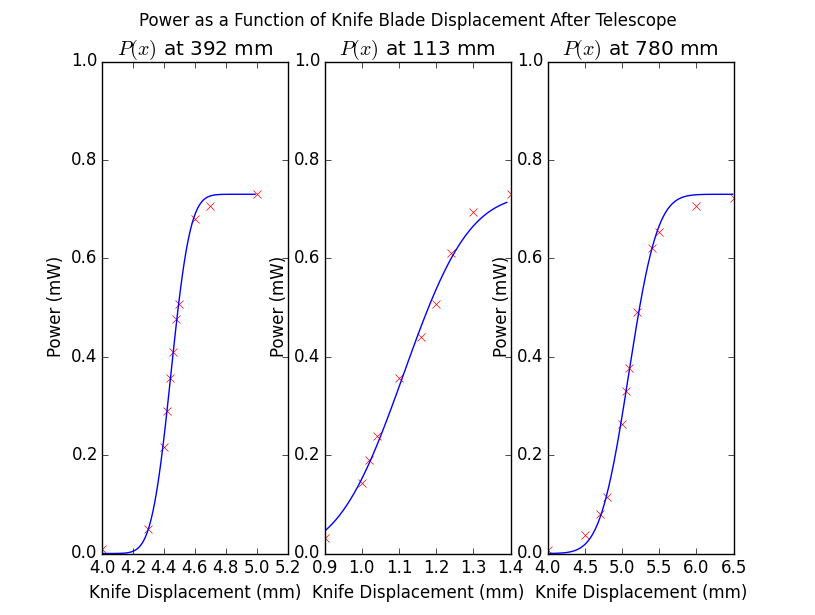
\includegraphics[scale=0.6]{../Analysis/beam_profile_after.png}
\caption{Red crosses are observed experimental, blue line is our fit.}
\end{figure}

From this, we fit the resulting values of $z$ (with the second mirror as our reference point) and $w({z})$ to the equation for the evolution of the beam i.e.

$$w(z)^{2} = w_{0}^{2}\left(1 - \left(\dfrac{z\lambda}{w_{0}^{2}n\pi}\right)^{2}\right)$$

with an additional offset $d$ included with $z$.
\begin{figure}[H]
\centering
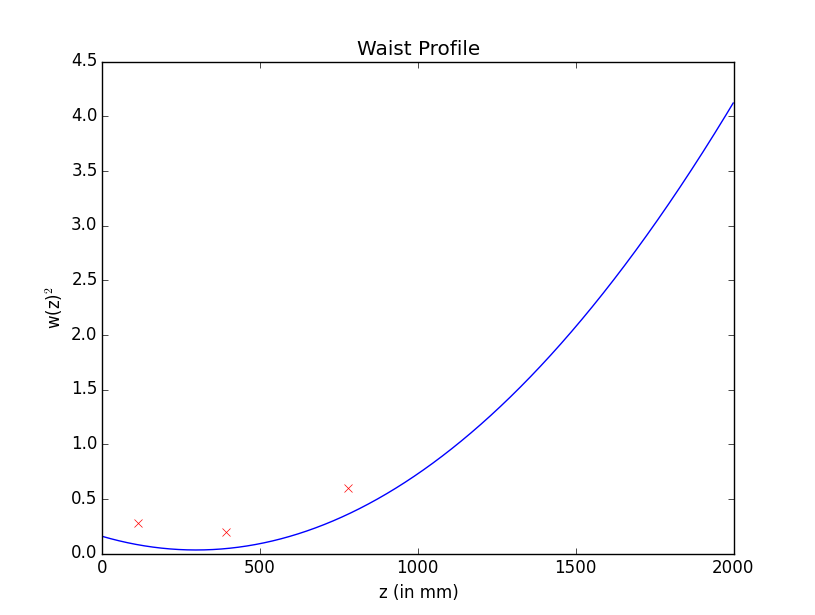
\includegraphics[scale=0.5]{../Analysis/waist_profile.png} 
\caption{Waist profile. Minimum is at 298 mm. Red crosses indicate observed data; blue line is the fit.}
\end{figure}
\end{itemize}
We choose to  place our collimator at about 300 mm, with sufficient margin to overlap at 298 mm. 
\section*{Part 3: Setup the Aspheric Lens}
We simply placed our collimator at the position of the minimum waist (the waist size was approximately 3 microns at that position) and attached our single-mode fiber optic to it. We walked the beam until the resulting light through the collimator was maximised.

\section*{Part 4: Tune the Fiber Coupling}
We cheated a little at this stage: we used a laser flashlight pen to progagate light backwards through the fiber optic and then tried to maximise its overlap with the incoming light. This strategy allowed us to achieve the most light going through than we had so far. 

\section*{Part 5: Measure the Out-Coupled Beam}
\begin{itemize}
\item Measure the total power coming through the fiber and calculate the fiber coupling efficiency you achieved (i.e. Power Out/Power In). How does this compare with what you expect based on your theoretical coupling efficiency?

\textbf{Answer: } The power coming in was measured to be 2.22 V (0.7 mW). The power going out of the two fiber couplings was 400 mV (or 0.13 mW). \\
\\
The efficiency is 
$$ \dfrac{\mathrm{Power\; Out}}{\mathrm{Power\; In}} = \dfrac{0.13}{0.7} = 0.18 = 18 \%$$

This is much smaller than my roughly calculated theoretical efficiency, which was about 75\%.

\item Observe the laser mode profile before and after the fiber. What differences do you see? Explain them.

\textbf{Answer: } The beam is (at least as a first approximation) apparently perfectly collimated along both axes, with lower intensity afterwards.

\item Observe the laser mode profile before and after the fiber. What differences do you see? Explain them.

\textbf{Answer: } The beam is (at least as a first approximation) apparently perfectly collimated along both axes, with lower intensity afterwards. The light is perfectly circular afterwards.

\item Insert a PBS into the out-coupled beam and measure the power in polarization. Is the power constant in time? 

\textbf{Answer: } The power through the polariser is exactly 200 mV (0.0625 mW) i.e. half of the power has been lost. This indicates that the light is circularly polarized. This power is constant in time - \textsl{assuming} the fiber optic is not being moved and is perfectly straight. See next question.

\item Try gently shaking the fiber (not the mounts!) and observe what happens to the power. Document and try to offer an explanation.

\textbf{Answer: }The power is no longer constant in time, but fluctuates roughly linearly with the degree of deviation of the fiber coupling from its original state. The implication is clear: light  is now elliptically polarized as it exits the fiber coupling. The reason for this 
\end{itemize}
\end{document}